\section{ Robotic Platform and Experimental Setup}
\label{sec:experimental_setup}



\begin{figure}
    \centering
    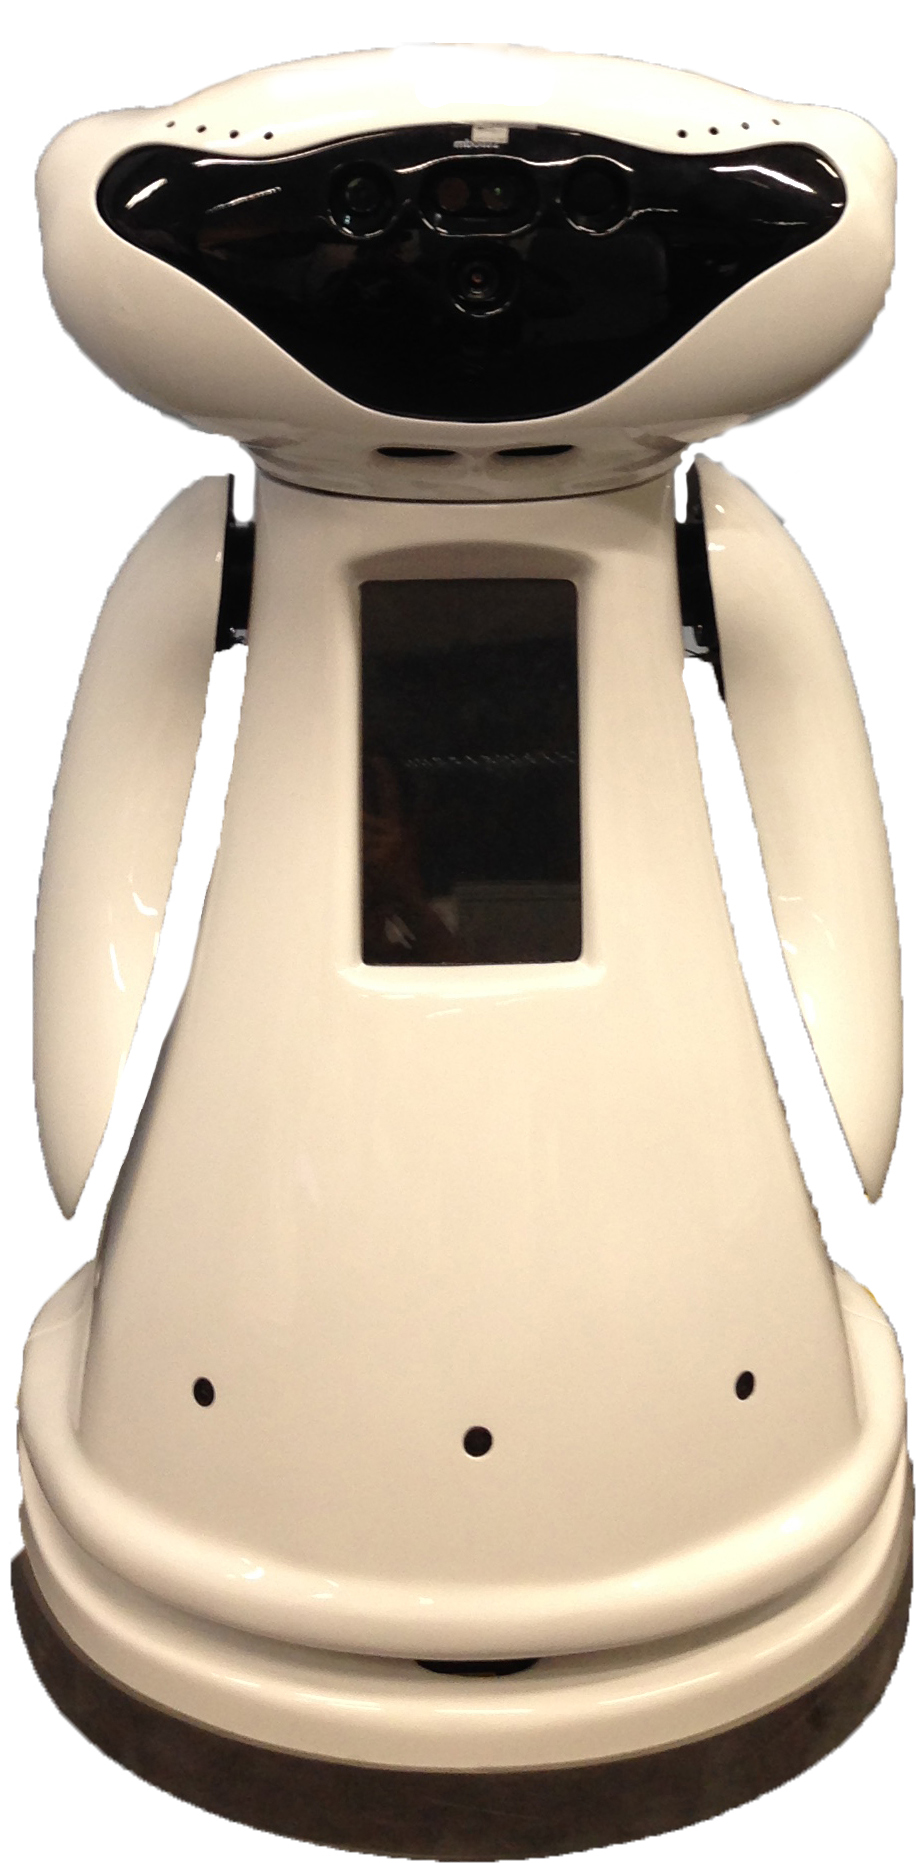
\includegraphics[scale=0.07]{pictures/robot.jpg}
    \caption{Robot used in our experiments to perform the automatic fingerprinting.}
     \label{robot}
\end{figure}

%\begin{figure}
%    \centering
%    \includegraphics[scale=0.4]{pictures/lrf.jpg}
%    \caption{Principle of operation of the laser range finders. Taken by: http://msdn.microsoft.com.}
%     \label{lrf}
%\end{figure}

\begin{figure}
    \centering
    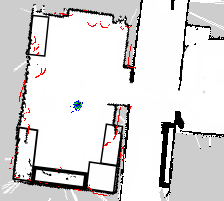
\includegraphics[scale=0.64]{pictures/amcl.png}
    \caption{Graphical view of the robot's position estimation with AMCL. The blue dot is the position estimate, while the red dots represent the measurements of the laser range finders.}
     \label{amcl}
\end{figure}


The robotic platform used in this work is shown in Figure \ref{robot}. This robot is called mBot \cite{Messias2014robotic} and is developed within the FP7 European project MOnarCH (Multi-Robot Cognitive Systems Operating in Hospitals \cite{monarch2013}).
It is an omni-directional drive robot with an approximately round footprint of 0.65m in diameter and a height of 0.98m.
It is provided with two laser range finders placed in the bottom of it, between the base and the rest of the robot, on both the front and the back for providing full coverage.

Two batteries give it an autonomy of approximately five hours, depending on the usage.
The robot has two PCs inside its shell: one manages the sensors, navigation and actuators, while the second one is for other functions such as human-robot interaction functionalities, which are outside our interests for this work.

The two on-board PCs, run Ubuntu desktop 12.04 and ROS Hydro. All the software modules that compose the underlying layers of the robotic platform were already implemented at the time of our work since the robot was already used in the context of the MOnarCH  project. These modules provide self localization and navigation capabilities, which are exposed through software interfaces to the user-level software.

The robot's self localization feature has fundamental importance in our work.
It is based on AMCL (Adaptive Monte Carlo Localization) \cite{amcl}, a probabilistic localization algorithm for a robot moving in 2D.
AMCL, a variation to the MCL above mentioned, provides an estimate of the position and orientation of the robot by matching the measurements of the laser range finders with a known map of the environment and considering the odometry data.

People detection and tracking is done by means of an omni-directional overhead camera (explain specifications) with x frames per second. The deterministic tracker outputs results with xx hz and the probabilistic tracker with y hz. (maybe a table for everything here)


Experiments are performed inside the robotics lab depicted in where the tracker is operational. Give dimensions of the room and tracker accuracy.


Ground truth position of the robot is given by AMCL with x accuracy and the person stands and walks on physically marked tracks to get the exact precise ground truth.


We study 4 scenarios for each of our human-aware navigation method each being tested 5 times.
We start with a single static person and incrementally increase the complexity to 2 moving people in the arena. We should emphasize that uncertainty is affecting the tracking performance and is not very evident from just looking at the environment. The person is not aware of what is happening on the tracker side, but the information given by the tracker greatly affects the behavior of the robot.



Figure shows a snapshot of the setup with two people moving in the arena. For the case of static people we have also done extensive tests using a high fidelity simulator webots \cite{michel1998webots}, by 1) emulating the uncertainty of tracking, and 2) replaying real uncertainty and tracking data from real experiments. This was done to simplify the debugging and speeding up the robotic tests.

Since we aim to study the effect of uncertainty and social factors in human-aware navigation we chose a task of point to point navigation for the robot in the vicinity of humans. The complexity of navigation task can be increased and more interesting scenarios in terms of HRI can be investigated but that is outside the scope of our work.


